\documentclass{article}
\usepackage[a4paper,bottom = 0.6in,left = 0.55in,right = 0.55in,top = 0.75in]{geometry}
\usepackage{graphicx}
\usepackage{amsmath}
\usepackage{array}
\usepackage{enumitem}
\usepackage{wrapfig}
\usepackage{titlesec}
\usepackage[colorlinks=false]{hyperref}
\usepackage{comment}
\usepackage{graphicx}

\newcommand{\xfilll}[2][1ex]{
\dimen0=#2\advance\dimen0 by #1
\leaders\hrule height \dimen0 depth -#1\hfill}
\titleformat{\section}{\large\scshape\raggedright}{}{0em}{}
\renewcommand\labelitemi{\raisebox{0.4ex}{\tiny$\bullet$}}
\renewcommand{\labelitemii}{$\cdot$}
\pagenumbering{gobble}
\begin{document}
% \vspace*{0 pt}
\noindent
\begin{minipage}{0.6\textwidth}
  \Large{Sourabh Singh} \\ \\
  \normalsize
  \begin{tabular}{p{7cm} p{30cm}}
  Computer Science and Engineering & B.Tech. \\
  Indian Institute of Technology, Bombay &  Male\\
  % Github & {https://github.com/ministark}\\
  Email: sourabhrishi25@gmail.com & DOB: 25/05/98 \\
  Contact: +919869815517 \\
  \end{tabular}
  % Department Computer Science and Engineering, IIT Bombay
\end{minipage}
\hfill 
\begin{minipage}{0.3\textwidth}\raggedleft
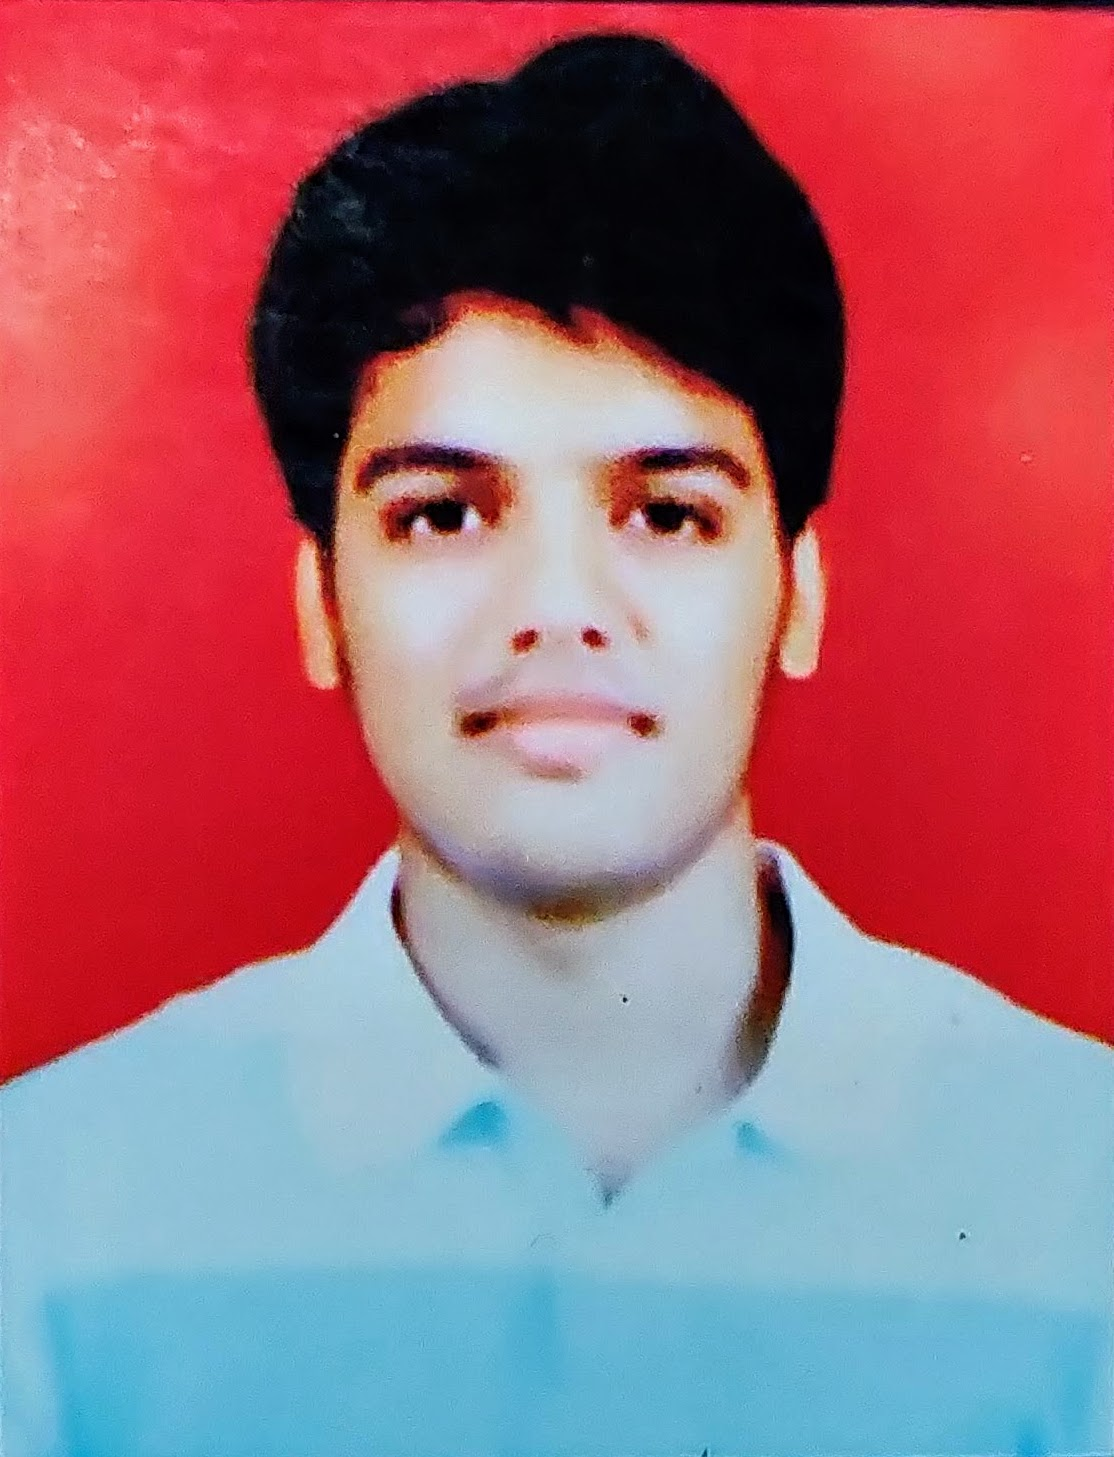
\includegraphics[width=0.5\linewidth]{./photo.jpg}
\end{minipage}

% \begin{figure}
%   \includegraphics[width=\linewidth]{../../Pictures/Rick&Morty.jpg}
%   \caption{A boat.}
%   \label{fig:boat1}
% \end{figure}

% \noindent{ \large
% \begin{tabular}{p{2cm} p{19cm}}
% Name & Sourabh Singh\\
% Github & {https://github.com/ministark}\\
% Email & sourabhrishi25@gmail.com\\
% Contact & +919869815517\\
% \end{tabular}
% }
% \vspace*{20 pt}

% \hspace {-15 pt} 
% Pursuing {\bf BTech} and {\bf Honours} degrees in Department Computer Science and Engineering\\
% \vspace*{-20 pt}
%%%%%%%%%%%%%%%%%%%%%%%%%%%%%%%%%%%%%%%%%%%%%%%%%%%%%%%Intern%%%%%%%%%%%%%%%%%%%%%%%%%%%%%%%%%%%%%%%%%%%%%%%%%%%%%%%%%%%%%%%%%%%%%%%%%%
\section*{{\LARGE Internships }\xfilll[0pt]{0.5pt}}
\vspace{-4pt}
\textbf{Risk Engine Development} \hfill{\sl \small May-June 2018}
  \vspace{1pt}\\
  { {Goldman Sachs} }\hfill{\sl \small Bengaluru}\\
  \vspace{-17pt}
  \begin{itemize}[itemsep = -0.75 mm, leftmargin=*]
      \item Designed infrastructure that reconciles 3 risk engines for over 10 risk measures; flagging inconsistent risk
      \item Developed book level service which computes risk using risk engine OGRE, scheduled daily for all portfolios
      \item Identified and resolved issues in Credit Risk Framework reducing inconsistency below 1\% for flagged tradables 
      \item Designed utilities to get summary report of all process running overnight and to manage containers in Database
  \end{itemize}
\textbf{Game Engine Development} \hfill{\sl \small May-June 2017}
  \vspace{1pt}\\
  { {Ubisoft} }\hfill{\sl \small Pune}\\
  \vspace{-17pt}
  \begin{itemize}[itemsep = -0.75 mm, leftmargin=*]
      \item Designed 2D Game engine from scratch in C++11 consisting of Rendering \& Physics Engine and State Manager 
      \item Developed Rendering Engine using \textbf{DirectX} besides HLSL for shaders providing more graphical elements 
      \item Optimised Physics Engine using Rvalue, Quadtrees for collision detection, and other inspirations from Box2D
      \item Implemented ideas from different Design Patterns like Factory, Singleton to create game with Haaf game engine
  \end{itemize}
\textbf{Software Development and Research Intern} \hfill{\sl \small December 2016}
  \vspace{1pt}\\
  { {Wellthy Therapeutics} }\hfill{\sl \small Mumbai}\\
  \vspace{-17pt}
  \begin{itemize}[itemsep = -0.75 mm, leftmargin=*]
      \item Engineered a raw chat system based on the \textbf{MQTT} protocol using \emph{Mosquitto} as a MQTT broker
      \item Analysed its efficency against traditional protocol based chat application provided by various companies 
      \item Implemented User-Agent assignment system with Amazon's \textbf{Dynamodb} database and other web services
  \end{itemize}
%%%%%%%%%%%%%%%%%%%%%%%%%%%%%%%%%%%%%%%%%%%%%%%%%%%%%%%%%%  PROJECTS  %%%%%%%%%%%%%%%%%%%%%%%%%%%%%%%%%%%%%%%%%%%%%%%%%%%%%%%%%%%%%%%%%
\section*{\LARGE Course Projects\xfilll[0pt]{0.5pt}}
\vspace{-4pt}
\textbf{Analysing Parallel Sorting Algorithms} \hfill{\sl \small Spring 2018}
  \vspace{1pt}\\
  {\it Guide: Prof. Sharat Chandan}\hfill{\sl \small IIT Bombay}\\
  \vspace{-17pt}
    \begin{itemize}[itemsep = -0.75 mm, leftmargin=*]
      \item Implemented bitonic sort in cuda and compared its speed with a 64 core distributed OpenMPI implementation 
      \item Analysed its efficiency for input sizes upto one billion achieving 1.6 times greater speedup than distributed
      \item Evaluated sequential version of Bitonic Sort algorithm against Quicksort and Introsort (STL Library uses it)
    \end{itemize}
\textbf{Aarohi - Music Generating bot} \hfill{\sl \small Spring 2017}
  \vspace{1pt}\\
  {\it Guide: Prof. Ganesh Ramakrishnaxn}\hfill{\sl \small IIT Bombay}\\
  \vspace{-17pt}
    \begin{itemize}[itemsep = -0.75 mm, leftmargin=*]
      \item Trained models using \textbf{Keras} to synthesize music using RNN with LSTM Cells to track long term patterns
      \item Dataset were MIDI files of Bach Chorales converted to Piano-Roll, a more structured and intutive format
      \item Analysed the melody using mathematical models like Chromograph, Tempograph, and Recurrence Matrix
    \end{itemize}
\textbf{Crafter - 3D Modelling Tool} \hfill{\sl \small Autumn 2017}
  \vspace{1pt}\\
  {\it Guide: Prof. Parag Chaudhary}\hfill{\sl \small IIT Bombay}\\
  \vspace{-17pt}
    \begin{itemize}[itemsep = -0.75 mm, leftmargin=*]
      \item Designed 3D modeller with utilities such as saving, reverting in OpenGL; modelled object with 250+ vertices
      \item Implemented animator which snaps primary frames; linearly interpolates the joints parameters to develop video
    \end{itemize}
\textbf{Echo - Messaging Application} \hfill{\sl \small Spring 2017}
  \vspace{1pt}\\
  {\it Guide: Prof. Varsha Apte}\hfill{\sl \small IIT Bombay}\\
  \vspace{-17pt}
    \begin{itemize}[itemsep = -0.75 mm, leftmargin=*]
      \item Designed a C++ chat application with socket programming and multithreading on Linux for only shell 
      \item Included features such as Online-Offline user, MultiUser Login, Last seen, and History of all conversations
      \item User interface was completely terminal based handled by \textbf{Ncurses} with different themes to choose from
    \end{itemize}
\textbf{ATM Controller - VHDL} \hfill{\sl \small Spring 2017}
  \vspace{1pt}\\
  {\it Guide: Prof. Supratik Chakraborty}\hfill{\sl \small IIT Bombay}\\
  \vspace{-17pt}
    \begin{itemize}[itemsep = -0.75 mm, leftmargin=*]
      \item Engineered a ATM Controller for FPGA board, capable to withdraw and deposit cash connected to server
      \item Server maintained account balances and imposed restriction on cash dispensed over TEA encrypted channel 
      \item Implemented \textbf{Least Recent Used} caching algorithm for transactions when contact with server fails
    \end{itemize}
\textbf{Feed'er - Time Table App} \hfill{\sl \small Autumn 2016}
  \vspace{1pt}\\
  {\it Guide: Prof. Sharat Chandran}\hfill{\sl \small IIT Bombay}\\
  \vspace{-17pt}
    \begin{itemize}[itemsep = -0.75 mm, leftmargin=*]
      \item Developed an andriod application to notifiy students for upcoming projects and assignment deadlines
      \item Designed a forum using Django for instructor to update assignments and collect realtime feedback from students 
    \end{itemize}
\begin{comment}
\textbf{Checkers} \hfill{\sl \small Autumn 2015}
  \vspace{1pt}\\
  {\it Guide: Prof. Varsha Apte}\hfill{\sl \small IIT Bombay}\\
  \vspace{-17pt}
    \begin{itemize}[itemsep = -0.75 mm, leftmargin=*]
      \item Built the Checkers game using \textbf{Simplecpp} library for User Interface and other graphical elements  
      \item Included Two-player and Single-player mode with an AI implemented using \textbf{first level depth} search
      \item Evaluated and displayed validity of moves, and suggested all possible moves for the player to play
    \end{itemize}
\end{comment}
% \newpage
% \vspace{ 50pt}
% \hspace{-18 pt}
% \textbf{Breakout Game} \hfill{\sl \small Autumn 2016}
%   \vspace{1pt}\\
%   {\it Guide: Prof. Sharat Chandran}\hfill{\sl \small IIT Bombay}\\
%   \vspace{-17pt}
%     \begin{itemize}[itemsep = -0.75 mm, leftmargin=*]
%       \item Modified version of the famous \emph{Breakout game}, consisting of attractive/repulsive magnets
%       \item Designed it in C++ using {\bf Box2D}, a Physics Simulation Engine
%       \item Implemented dynamic memory allocation for improving runtime efficiency
%     \end{itemize}
% \textbf{Movie Recomendation Engine} \hfill{\sl \small Autumn 2016}
%   \vspace{1pt}\\
%   {\it Guide: Prof. Sharat Chandran}\hfill{\sl \small IIT Bombay}\\
%   \vspace{-17pt}
%     \begin{itemize}[itemsep = -0.75 mm, leftmargin=*]
%       \item Developed a movie recommendation engine in {\bf Python} using collaborative filtering technique
%       \item Primarily using \emph{Euclidian distance} and \emph{Pearson Correlation} to find the most relevant movies
%       \item Based on the input preferences of user, pool of movies and your ratings, movies are recommended to users 
%     \end{itemize}
%%%%%%%%%%%%%%%%%%%%%%%%%%%%%%%%%%%%%%%%%%%%%%%%%%%%%%%%%%  SCHOLASTIC ACHIEVEMENTS %%%%%%%%%%%%%%%%%%%%%%%%%%%%%%%%%%%%%%%%%%%%%%%%%%%%%%%%%%%%%%%%%%%%%
\section*{{\LARGE Scholastic Achievements}\xfilll[0pt]{0.5pt}}
\vspace{-4pt}
\begin{itemize}[itemsep = -0.75 mm, leftmargin=*]
    % \item Secured {\bf All India Rank 599} in JEE Advanced amongst 150,000 candidates \hfill {\sl \small 2015}
    
    \item Recipient of the Kishore Vaigyanik Protsahan Yojana Scholarship with \textbf{All India Rank 88}  \hfill \emph{\sl \small 2013}

    % \item Achieved {\bf 99.99} percentile in JEE Main out of 1.4 million candidates \hfill {\sl \small 2015}
        
    \item Succesfully cleared \textbf{Indian National Mathematics Olympiad} twice \hfill {\sl \small 2012, 2013}

    \item Awarded National Talent Search Examination Scholarship being among \textbf{top 1000} all over India \hfill {\sl \small 2012}

    % \item Participated in National Science \textbf{VIJYOSHI} camp organized by KVPY \hfill {\sl \small 2014}    

\end{itemize}
\vspace{-10pt}
% %%%%%%%%%%%%%%%%%%%%%%%%%%%%%%%%%%%%%%Interest%%%%%%%%%%%%%%%%%%%%%%%%%%%%%%%%%%%%%%%%%%5
% \section*{{\LARGE Interests}\xfilll[0pt]{0.5pt}}
% \vspace{-4pt}
% Network Security, Data Structures and Algorithms, Software Development, Machine learning, Cryptography, Graph Theory


%%%%%%%%%%%%%%%%%%%%%%%%%%%%%%%%%%%%%%%%%%%%%%%%%%%%%%%%%%%%%%%%%%%%%%%%%%%%%%%%%%%%%%%%%%%%%%%%%%%%%%%%%%%%%%%%%%%%%%%%%%%%%%%%%%%%%
\section*{\LARGE Technical Projects\xfilll[0pt]{0.5pt}}
\vspace{-4pt}
\textbf{FirstPersonShooting Game} \hfill{\sl \small Summer 2016}\\
  \vspace{-17pt}
    \begin{itemize}[itemsep = -0.75 mm, leftmargin=*]
      \item Developed multiplayer game inspired by CounterStrike with {\bf Unity5} game engine and {\bf C\#} scripting language 
      \item Introduced real life animations from first person perspective; multiplayer support for upto 16 players on internet
    \end{itemize}
% \textbf{Movie Recomendation Engine} \hfill{\sl \small Autumn 2016}
%   \vspace{-17pt}\\
%     \begin{itemize}[itemsep = -0.75 mm, leftmargin=*]
%        \item Developed a movie recommendation engine in {\bf Python} using collaborative filtering technique
%        \item Primarily using \textbf{Euclidian distance} and \textbf{Pearson Correlation} to find the most relevant movies
%       \item Based on the input preferences of user, pool of movies and your ratings, movies are recommended to users 
%     \end{itemize}
\textbf{Line Follower} \hfill{\sl \small Spring 2016}
  \vspace{-17pt}\\
    \begin{itemize}[itemsep = -0.75 mm, leftmargin=*]
      \item Bot with Differential Steering, IR sensors for detecting orientation, and AVR  microcontroller for Path correction
      \item Secured {\bf Second Position} in the competition conducted by Robotics Club, IIT Bombay
    \end{itemize}
% \textbf{Tanks} \hfill{\sl \small Autumn 2016}
%   \vspace{-4pt}
%     \begin{itemize}[itemsep = -0.75 mm, leftmargin=*]
%       \item 3D replication of famous game Tank in Unity each player has a tank that can fire shell any direction it wants
%       \item Shell explosion imitation and third person dynamic camera that auto-resizes to include both players in screen
%     \end{itemize}
\textbf{Miscellaneous} 
  \vspace{-4pt}
    \begin{itemize}[itemsep = -0.75 mm, leftmargin=*]
      \item Developed  movie recommendation engine in {\bf Python} using \textbf{Euclidian distance} and \textbf{Pearson Correlation}
      \item 3D replication of famous game Tank in Unity each player has a tank that can fire shell any direction it wants
      % \item {\bf Bluetooth Control Bot}: A bot controlled by app via bluetooth module, with 12V battery and 4-wheel drive
      % \item  Modified version of the famous Breakout game, consisting of attractive/repulsive magnets using Box2D
    \end{itemize}

%%%%%%%%%%%%%%%%%%%%%%%%%%%%%%%%%%%%%%%%%%%%%%%%%%%%%%   Position of Responsibility   %%%%%%%%%%%%%%%%%%%%%%%%%%%%%%%%%%%%%%%%%%%%%%%%%%%%%%%

\section*{\LARGE Position of Responsibility\xfilll[0pt]{0.5pt}}
\vspace{-4pt}
\textbf{Mentor - Department Academic Mentorship Programme (DAMP)} \hfill{\sl \small 2018, 2019}
  \vspace{1pt}\\
    {\it Selected to be part of 23-member team among 100 applicants based on strong interpersonal skills and peer reviews}\\
    \vspace{-17pt}
      \begin{itemize}[itemsep = -0.75 mm, leftmargin=*]
        \item Mentoring 7 sophomores with diverse academic standing with their academic and co-curricular pursuits
        \item Guiding 2 students to help them clear their backlogs as a part of Academic Rehabilitation Programme (ARP)
      \item Coordinating with faculty advisor and course instructors to aid academically underperforming students
    \end{itemize}


%%%%%%%%%%%%%%%%%%%%%%%%%%%%%%%%%%%%%%%%%%%%%%%%%%%%%%  TECHNICAL SKILLS   %%%%%%%%%%%%%%%%%%%%%%%%%%%%%%%%%%%%%%%%%%%%%%%%%%%%%%%

\section*{\LARGE Technical Skills\xfilll[0pt]{0.5pt}}
\vspace{-4pt}
\begin{tabular}{p{3cm} p{13.5cm}}
    \textbf{Programming} &C, C++, Java, Python, Bash, SQL, HLSL, C\#, R ,VHDL, Django, Spring Framework\\ \\
    \textbf{Softwares} &Git, Unity3D, UnrealEngine, Andriod Studio, DirectX, OpenGL, \LaTeX, Wireshark\\
\end{tabular}


%%%%%%%%%%%%%%%%%%%%%%%%%%%%%%%%%%%%%%%%%%%%%%%%%%%%%%%%  KEY COURSES UNDERTAKEN   %%%%%%%%%%%%%%%%%%%%%%%%%%%%%%%%%%%%%%%%%%%%%%%%%%%

\section*{\LARGE Key Courses \xfilll[0pt]{0.5pt}}
\vspace{-4pt}
\hspace{-8pt}
  \begin{tabular}{p{30mm} p{14cm}}
  	\textbf{Theoretical CS} &Parallel Programming Paradigm, Artificial Learning, Introduction to Machine Learning, Automata Theory, Computer Graphics, Digital Image Processing \\
    \vspace{0.5 mm}\textbf{Systems} & \vspace{0.5 mm} Operating Systems, Computer Architecture, Cryptography and Network Security \\
  \end{tabular}
  \vspace{-3pt}\\
  % \hspace*{120mm}{\sl *{\it to be completed by November 2018}}
  % \hspace*{120mm}{\sl **{\it to be completed by April 2017}}
\vspace{-5pt}

%%%%%%%%%%%%%%%%%%%%%%%%%%%%%%%%%%%%%%%%%%%%%%%%%%%%%%%%%%%  EXTRACURRICULARS   %%%%%%%%%%%%%%%%%%%%%%%%%%%%%%%%%%%%%%%%%%%%%%%%%%%%%%
\section*{\LARGE Extracurriculars\xfilll[0pt]{0.5pt}}
\vspace{-4pt}
\begin{itemize}[itemsep = -0.75 mm, leftmargin=*]
  \item Completed course to learn Elementary German (\emph{Deutsch}) 
  % \item Participated in Microsoft's \textbf{Code.Fun.Do} boot camp with a game built using Unity5
  % \item Designed a responsive website using Materialize templates and HTML5 with on the fly form validation 
  % \item Engineered an aeromodel with pusher configuration for RC plane competition
  \item Swam \textbf{20.4 km} in 12hrs in the Swimmathon; part of Institute's Waterpolo Team for Inter-IIT 2018-19
  % \item Partcipated in Waterpolo GC, SwimmingGC and all other events conducted by IITB Aquatics Club
  \item Instructed and performed at Institute Salsa Night, 2016 with an audience of 1000+ people
  \item Showcased dance performances in the Annual InSync Dance Show, 2017 in front of 3000+ audience
\end{itemize}

\end{document}\grid
\grid
\grid
\grid
\grid
\grid
\grid
